\section{Aufgabe 3}
\subsection{Aufgabe 3 a)}
Eine Visualisation ist in \ref{fig:iso} zu sehen. 
\begin{figure}
    \centering
    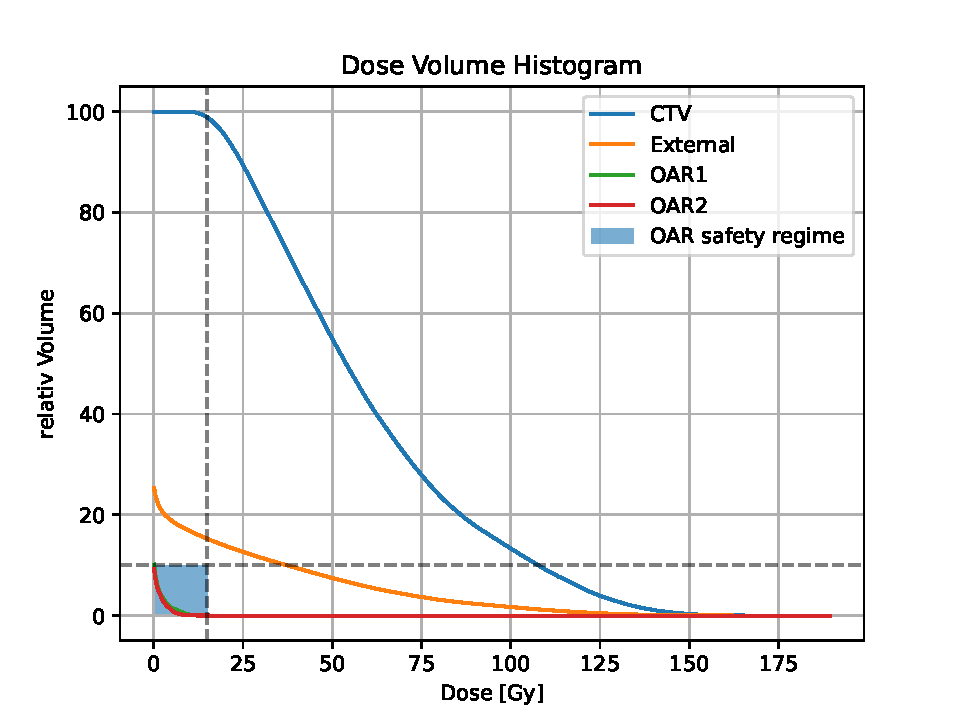
\includegraphics[width  = 0.8\textwidth]{content/DVH.pdf}
    \caption{Abgebildet ist ein Dosis Volumen Histogram eines klinischen Volumen und zwei Risikoorgane.}
    \label{fig:dvh}
\end{figure}
Deutliche Probleme des Plans sind die Fehlbarkeiten hinsichtlich der $95\% / 107\%$ Regel die nicht eingehalten wurden \ref{fig:slicer}.

\subsection{Aufgabe 3 b)}
Potentielle Unischerheiten in der Protonentherapie sind vorallem Dichte Anomalien hinsichtlich des Braggpeaks. 
Dieser Peak wurde in disem Projekt jedoch nicht benutzt, bzw. er liegt weit hinter dem CTV. Bei klinischer Anwenung wird der Peak jedoch ausgenutzt
um im Tumorvolumen geziehlt viel Dosis zu deponieren. Bei, im CT nicht auftretenden, Strukturen aus Luft wird so der Peak drastisch verschoben 
und die Dosis richtet so eventuell großen Schaden in Risikoorganen an. Dem lässt sich durch Vielfelder Pläne entgegenwirken da so 
eizelne Felder nicht mehr von großer Potenz sind und die Dosis homogener verteilt wird.